\documentclass[12pt]{article}\pagestyle{myheadings}
\usepackage{graphicx}
\usepackage{placeins}
\usepackage{float}
\textwidth 7.0 truein
\oddsidemargin -0.25in   %left-hand edge
\evensidemargin -0.5 truein  %right-hand edge
\topmargin -0.85in      %top of paper to top of head, pulls whole unit
\textheight 9.5in

%Enter your last name, the portfolio problem number, and the draft number.
\title{Homework 3 \\ Chaotic Dynamics - CSCI 4446}
\author{Denis Kazakov}
\date{February 1, 2015}


\usepackage{amsmath,amssymb,amsthm,amsfonts,graphicx}
%The following commands allow us to typeset theorems, propositions, definitions, etc.
\theoremstyle{plain}
\newtheorem{theorem}{Theorem}
\newtheorem{lemma}[theorem]{Lemma}
\newtheorem{corollary}[theorem]{Corollary}
\newtheorem{proposition}[theorem]{Proposition}
\newtheorem*{definition}{Definition}

\renewcommand{\qedsymbol}{\ensuremath{\blacksquare}}
\newcommand{\N}{\mathbb{N}}
\newcommand{\Z}{\mathbb{Z}}
\newcommand{\Q}{\mathbb{Q}}
\newcommand{\R}{\mathbb{R}}
\newcommand{\C}{\mathbb{C}} 
\begin{document}
\maketitle


\section{}

Our system is:	
$ml \ddot{\theta} + \beta l \dot{\theta} + mg\sin{\theta} = A \cos{\alpha t}$

\section{}

\subsection{a}	
\begin{figure}[H]
\centering
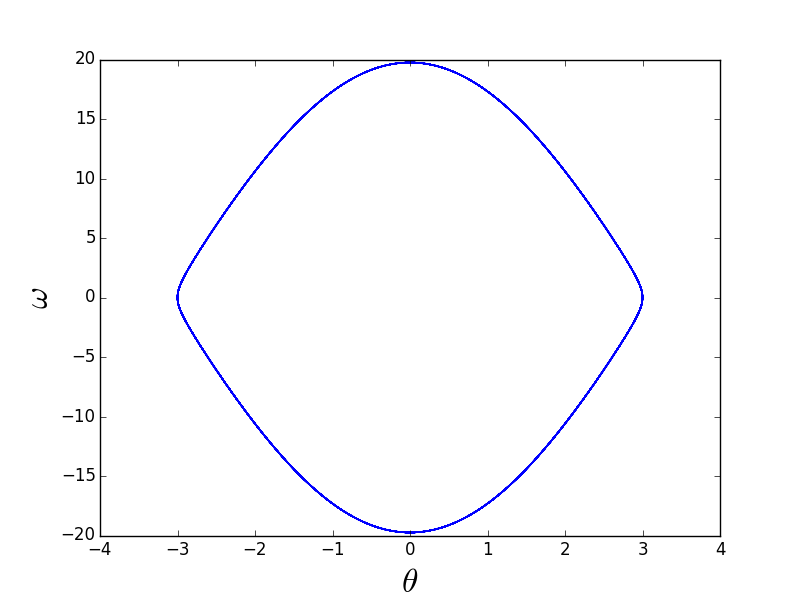
\includegraphics[scale=.25]{2a}
\caption{[$\theta$, $\omega$] = [3, 0.1], using $g = 9.8$, $\beta = 0.0$, $m = 0.1$, $l = 0.1$,$\alpha = 0.0$, $A = 0.0$}
\label{fig:my_label}
\end{figure}

This initial condition is near the unstable equilibrium point of [$\theta$, $\omega$] = [$\pi$, 0.0], where $\theta = \pi$ is at the top-most point of our pendulum's trajectory. 

\subsection{a}	
\begin{figure}[H]
\centering
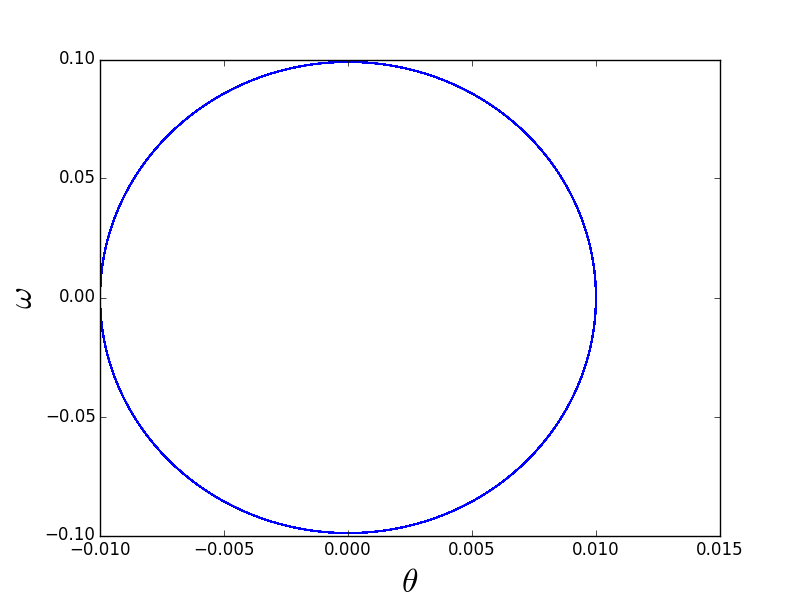
\includegraphics[scale=.25]{2b}
\caption{[$\theta$, $\omega$] = [0.01, 0.0], using $g = 9.8$, $\beta = 0.0$, $m = 0.1$, $l = 0.1$,$\alpha = 0.0$, $A = 0.0$}
\label{fig:my_label}
\end{figure}

This initial condition makes our state-space trajectory look much more like a perfect ellipse. This happens because as $\theta \to 0$, our pendulum starts behaving more and more like a simple spring oscillator, where difference in angle doesn't make a difference in the gravitational force. As  $\theta$ grows bigger, the difference coming from ($\sin{\theta}$) in the expression ($mg\sin{\theta}$) becomes more and more noticeable. 


\section{}

\begin{figure}[H]
\centering
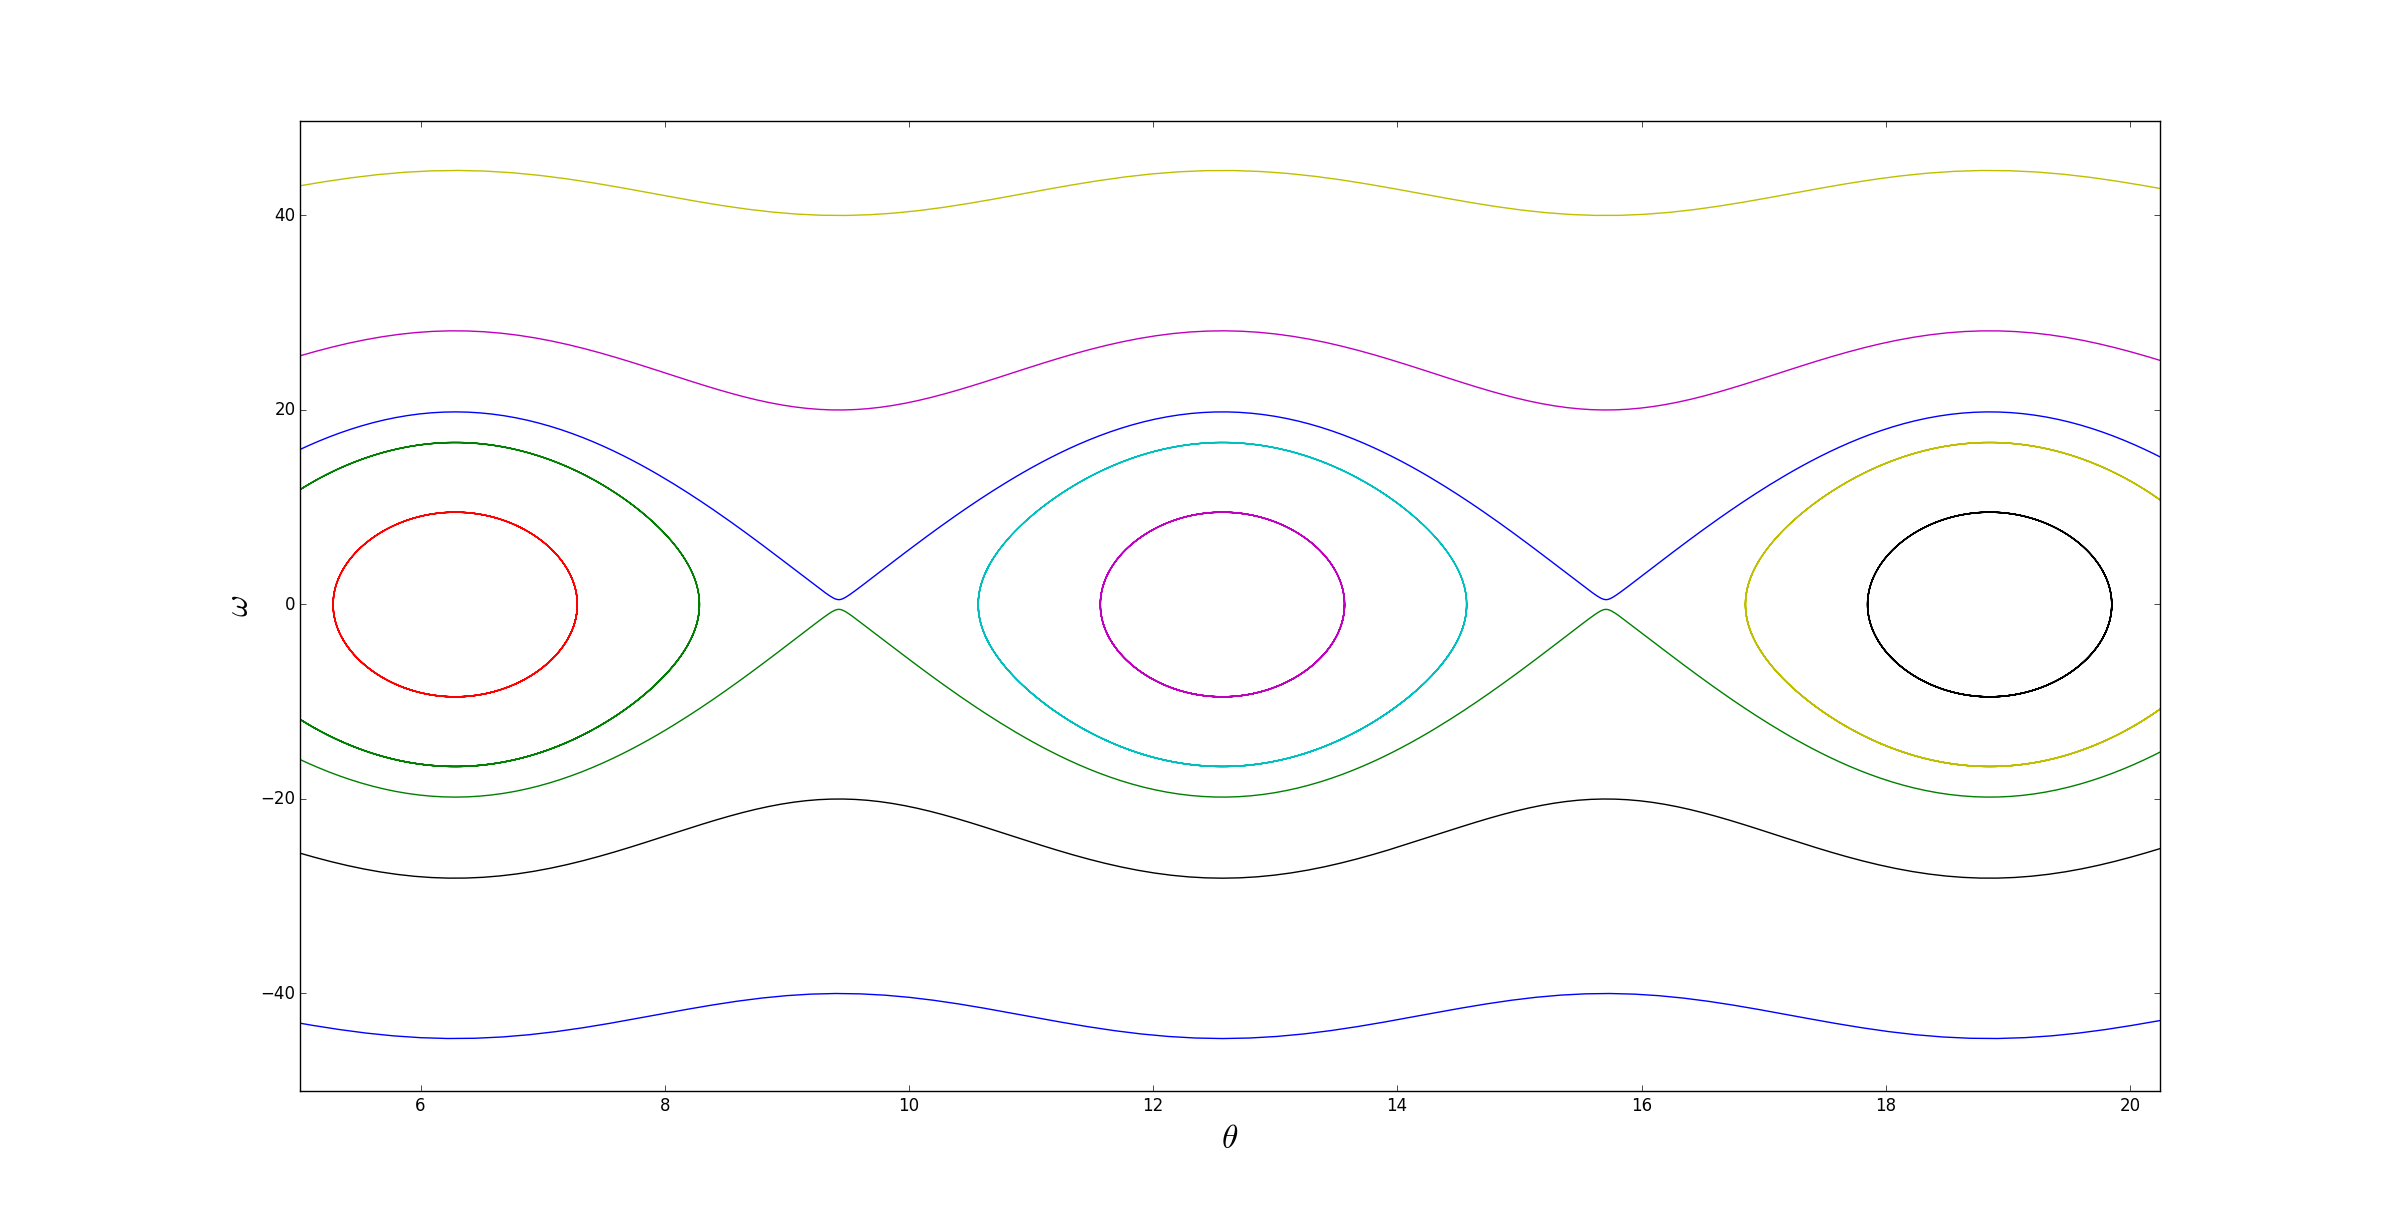
\includegraphics[scale=.15]{3}
\caption{state-space portrait using $g = 9.8$, $\beta = 0.0$, $m = 0.1$, $l = 0.1$,$\alpha = 0.0$, $A = 0.0$}
\label{fig:my_label}
\end{figure}

To capture all salient behavior of the pendulum's oscillation, we have to remember that pendulum has two principal types:
\begin{enumerate}
\item oscillating back and forth between a certain range of $\theta$
\item spinning at high enough speed that it doesn't oscillate back, instead only propagating forward/backward.
\end{enumerate}

Accordingly, we choose points that capture those 2 types of behavior and show how perturbations in conditions affect the state-space trajectory. 

\section{}

\begin{figure}[H]
\centering
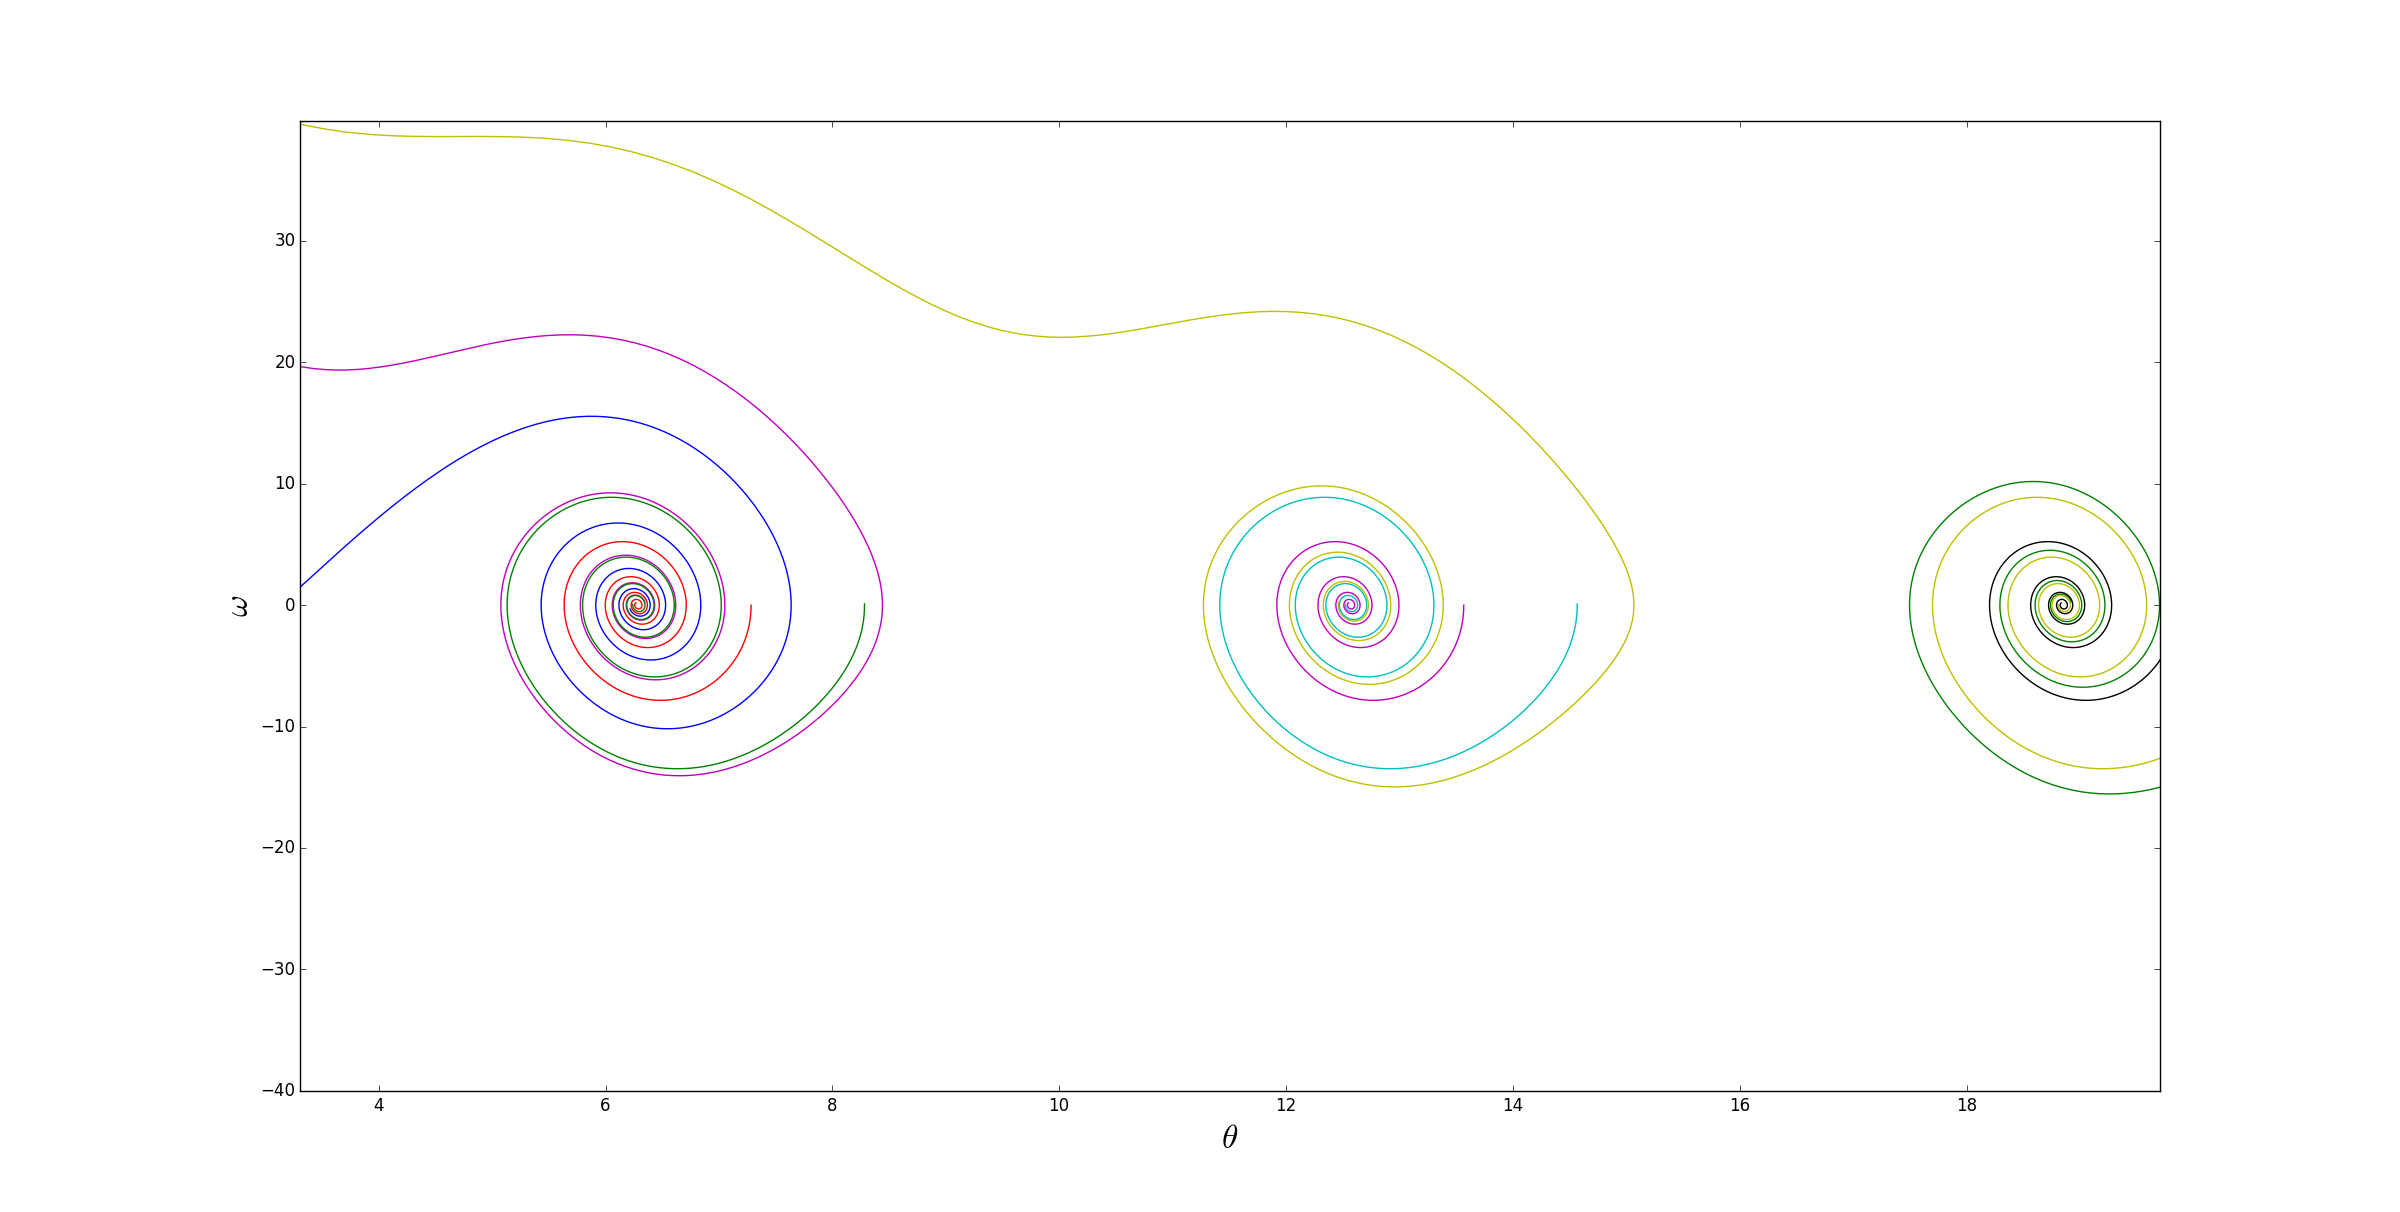
\includegraphics[scale=.15]{4}
\caption{state-space portrait using $g = 9.8$, $\beta = 0.25$, $m = 0.1$, $l = 0.1$,$\alpha = 0.0$, $A = 0.0$}
\label{fig:my_label}
\end{figure}

We see that now state-space trajectories converge to stable equilibrium points that are located at the "bottom" of our pendulum's trajectory ($\theta = 0 + 2\pi n, n \in \mathbb{Z}$).

In our model, $\beta$ is responsible for dampening the motion of our pendulum. Therefore, we expect that for higher $\beta$, trajectories will converge faster, and for smaller $\beta$, trajectories, will converge slower. 

Indeed, that can be easily verified by using smaller $\beta$ value:

\begin{figure}[H]
\centering
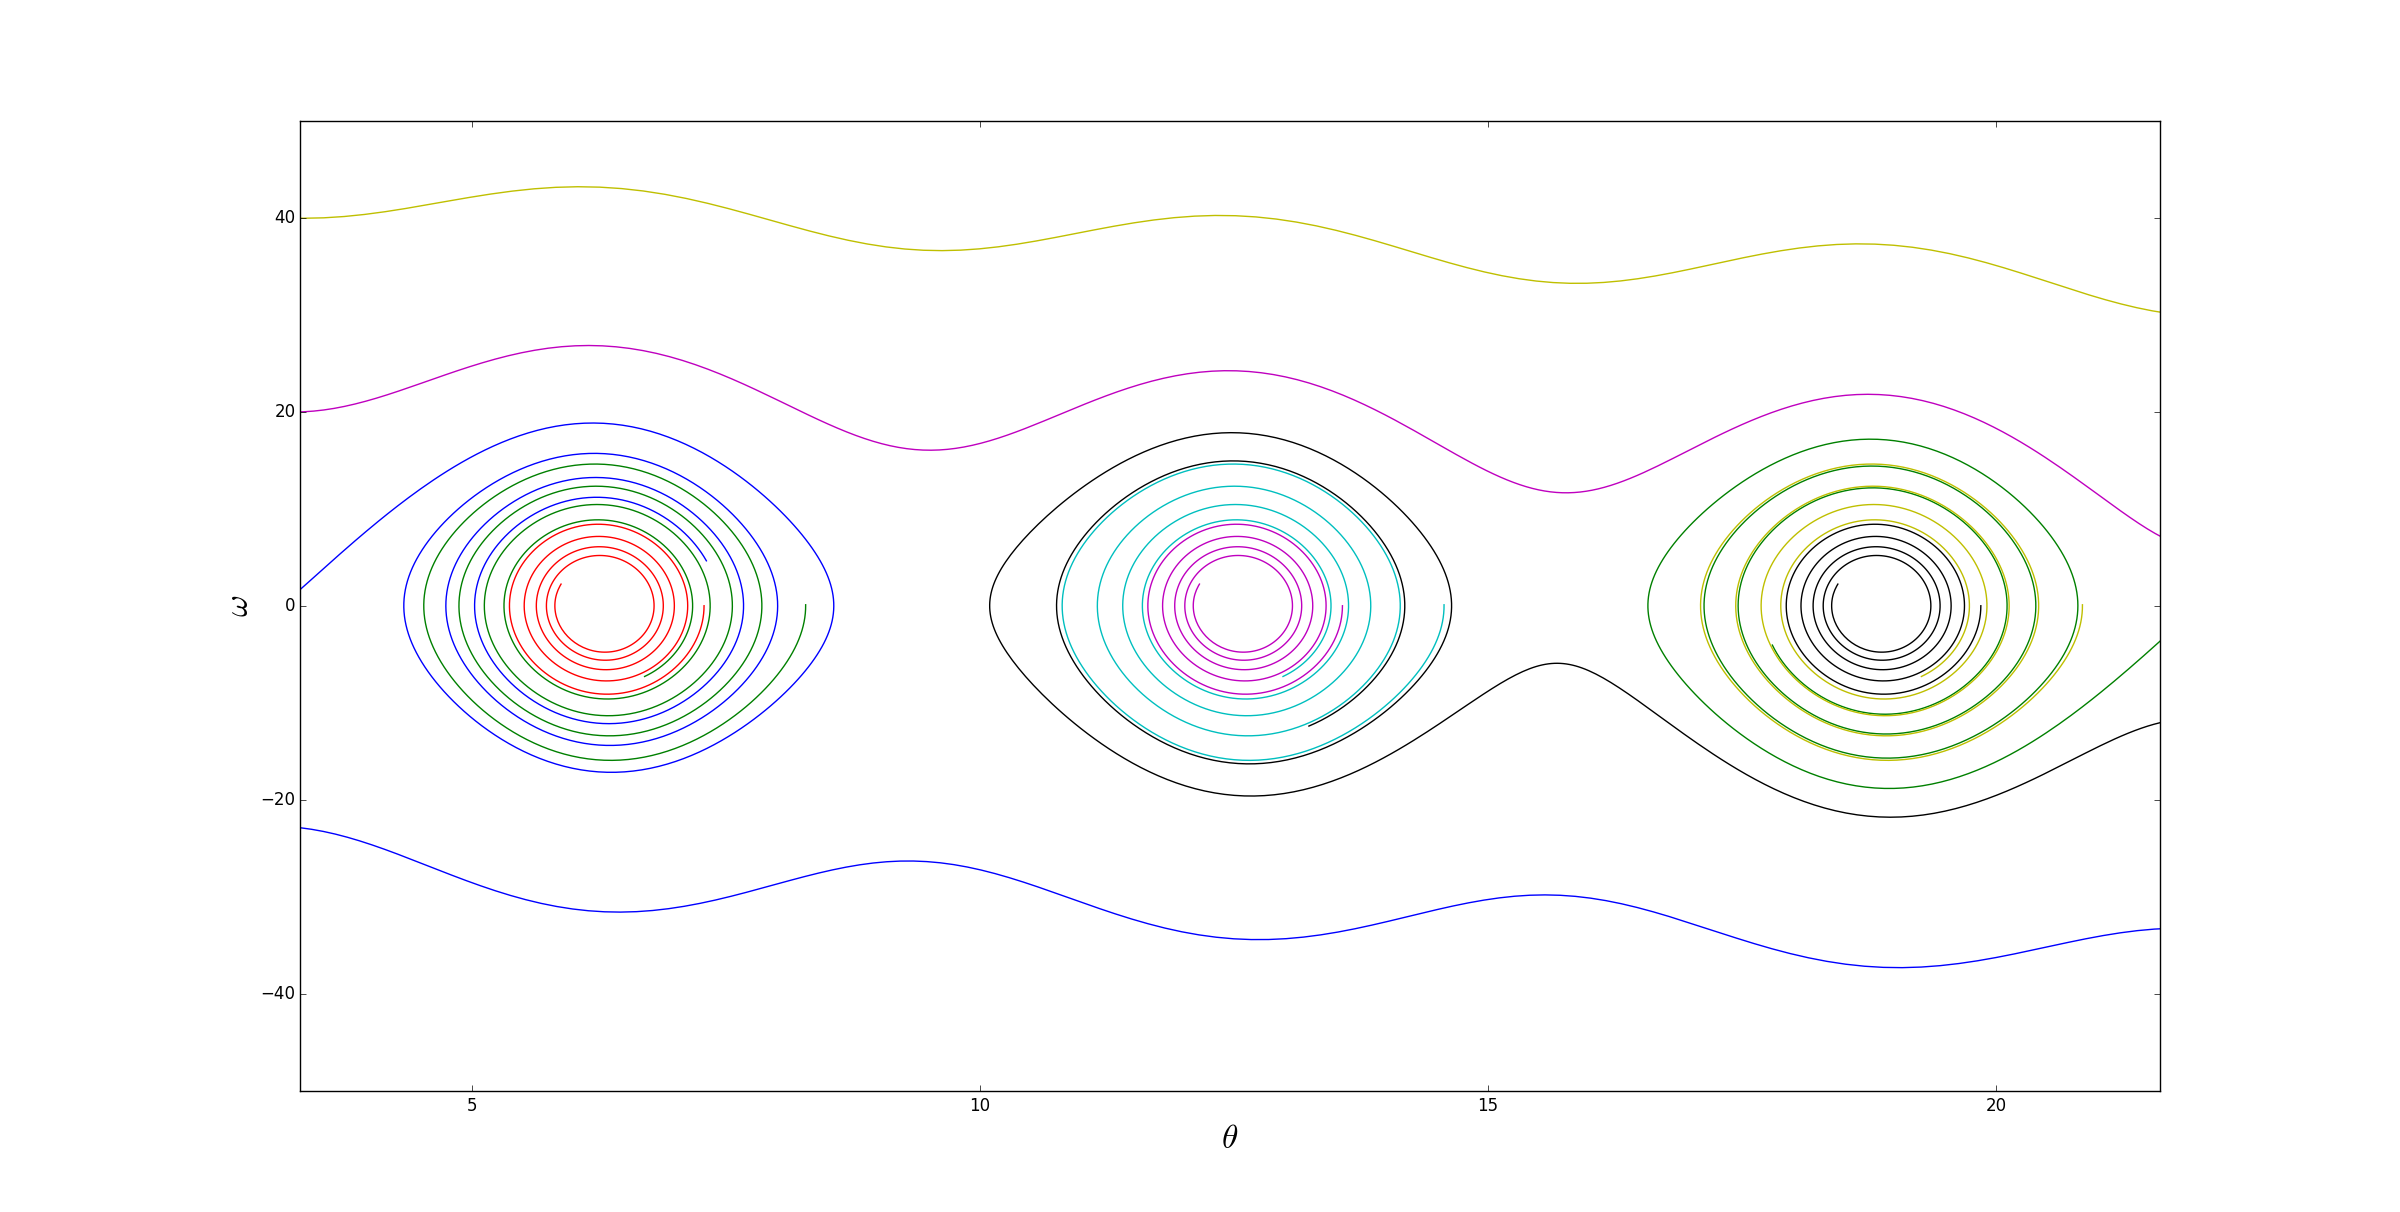
\includegraphics[scale=.15]{4extra}
\caption{state-space portrait using $g = 9.8$, $\beta = 0.05$, $m = 0.1$, $l = 0.1$,$\alpha = 0.0$, $A = 0.0$}
\label{fig:my_label}
\end{figure}

We see how trajectories "stay around" for longer in this plot. 

\section{}

\begin{figure}[H]
\centering
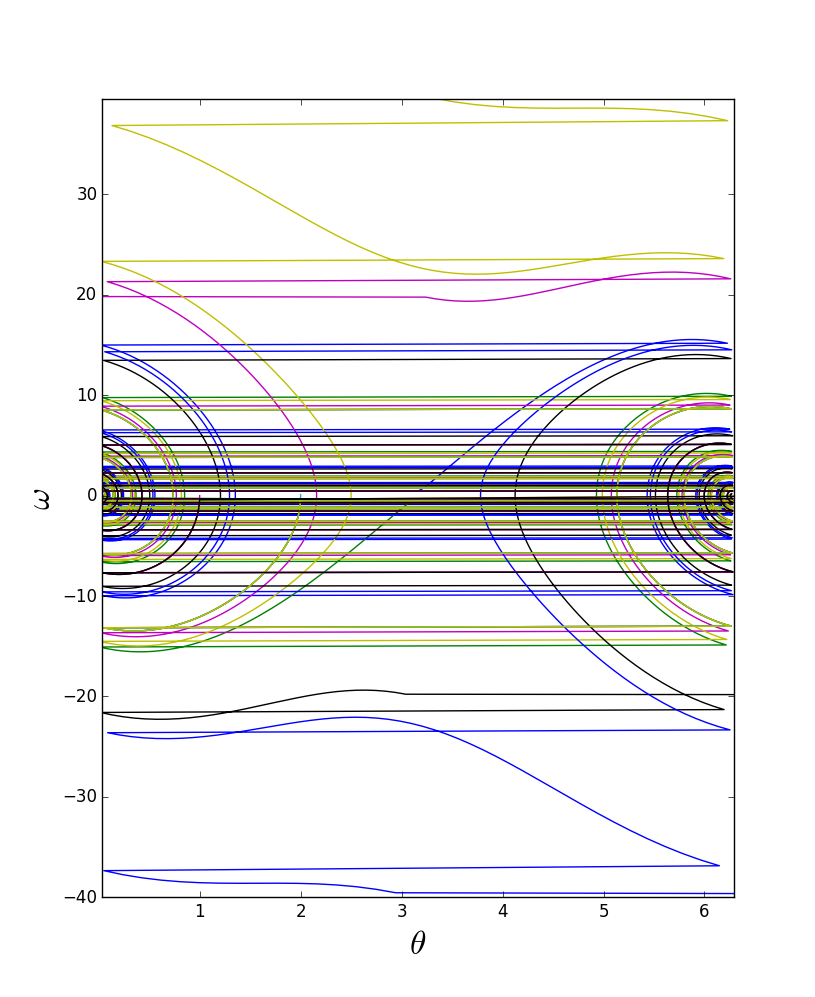
\includegraphics[scale=.3]{5}
\caption{state-space portrait modulo $2\pi$ using $g = 9.8$, $\beta = 0.05$, $m = 0.1$, $l = 0.1$,$\alpha = 0.0$, $A = 0.0$}
\label{fig:my_label}
\end{figure}

We can interpret this image as us overlaying all the periods of dampened pendulum oscillations on the range of $[0, 2\pi]$. This makes trajectories layer on top of each other. horizontal lines that we see are just a result of taking modulus on the $\theta$ and then plotting those coordinates as a continuous line. 

\section{}

Let's make bifurcation plots as we change $\alpha$ at $A = 1.15$.

\begin{figure}[H]
\centering
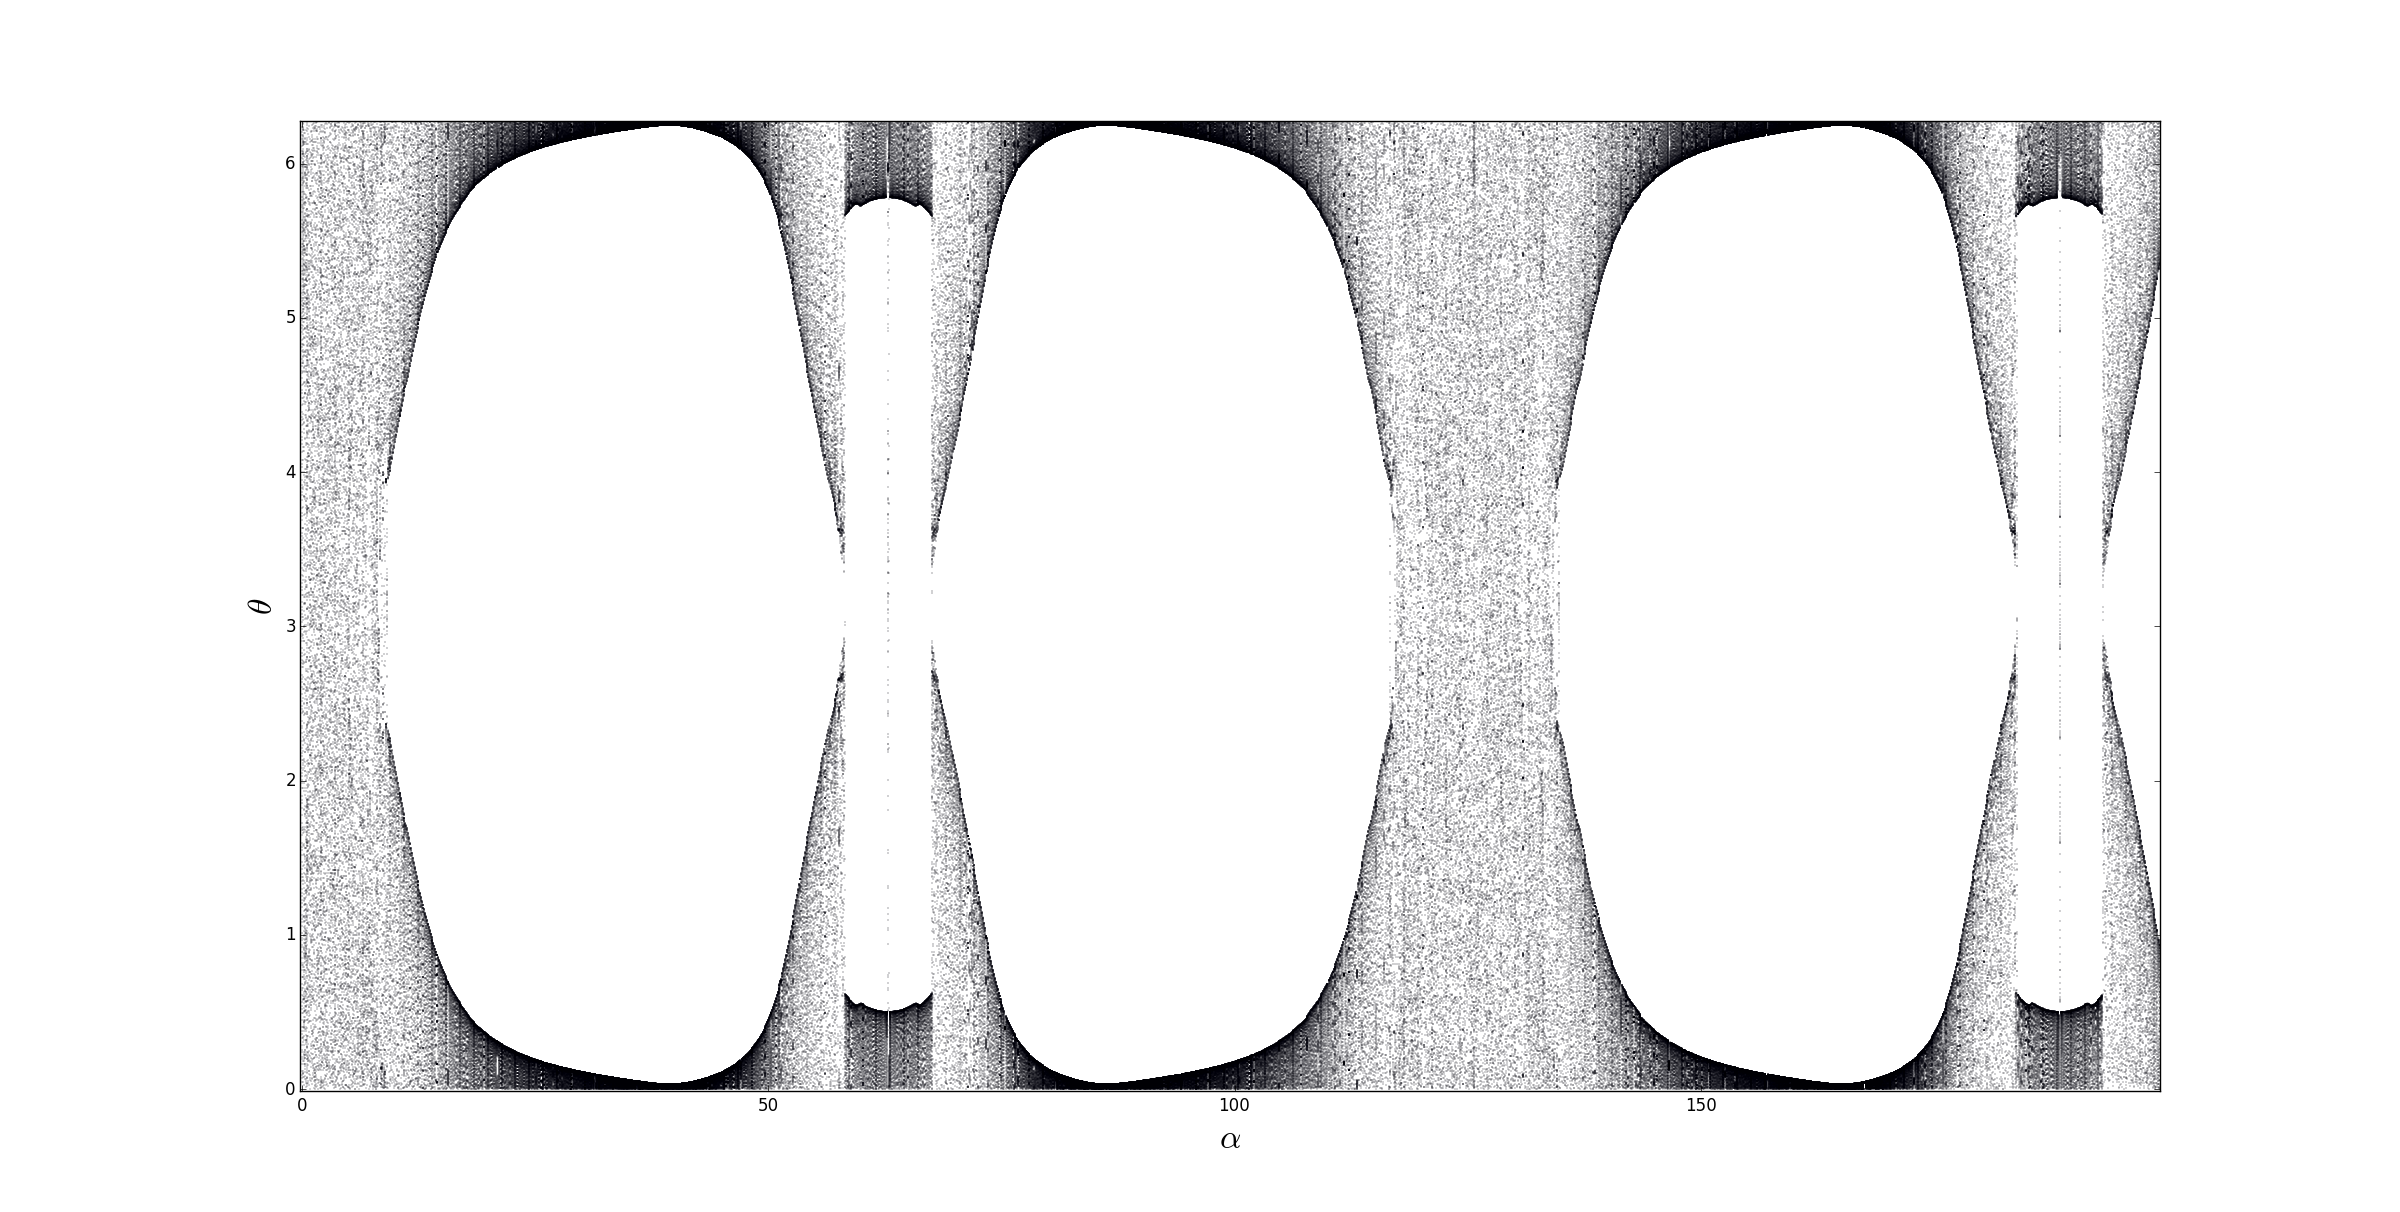
\includegraphics[scale=.25]{6_theta}
\caption{bifurcation plot of $\theta$  $g = 9.8$, $\beta = 0.0$, $m = 0.1$, $l = 0.1$,$\alpha \in [0,200]$, $A = 1.15$, step size = $0.01$}
\label{fig:my_label}
\end{figure}

\begin{figure}[H]
\centering
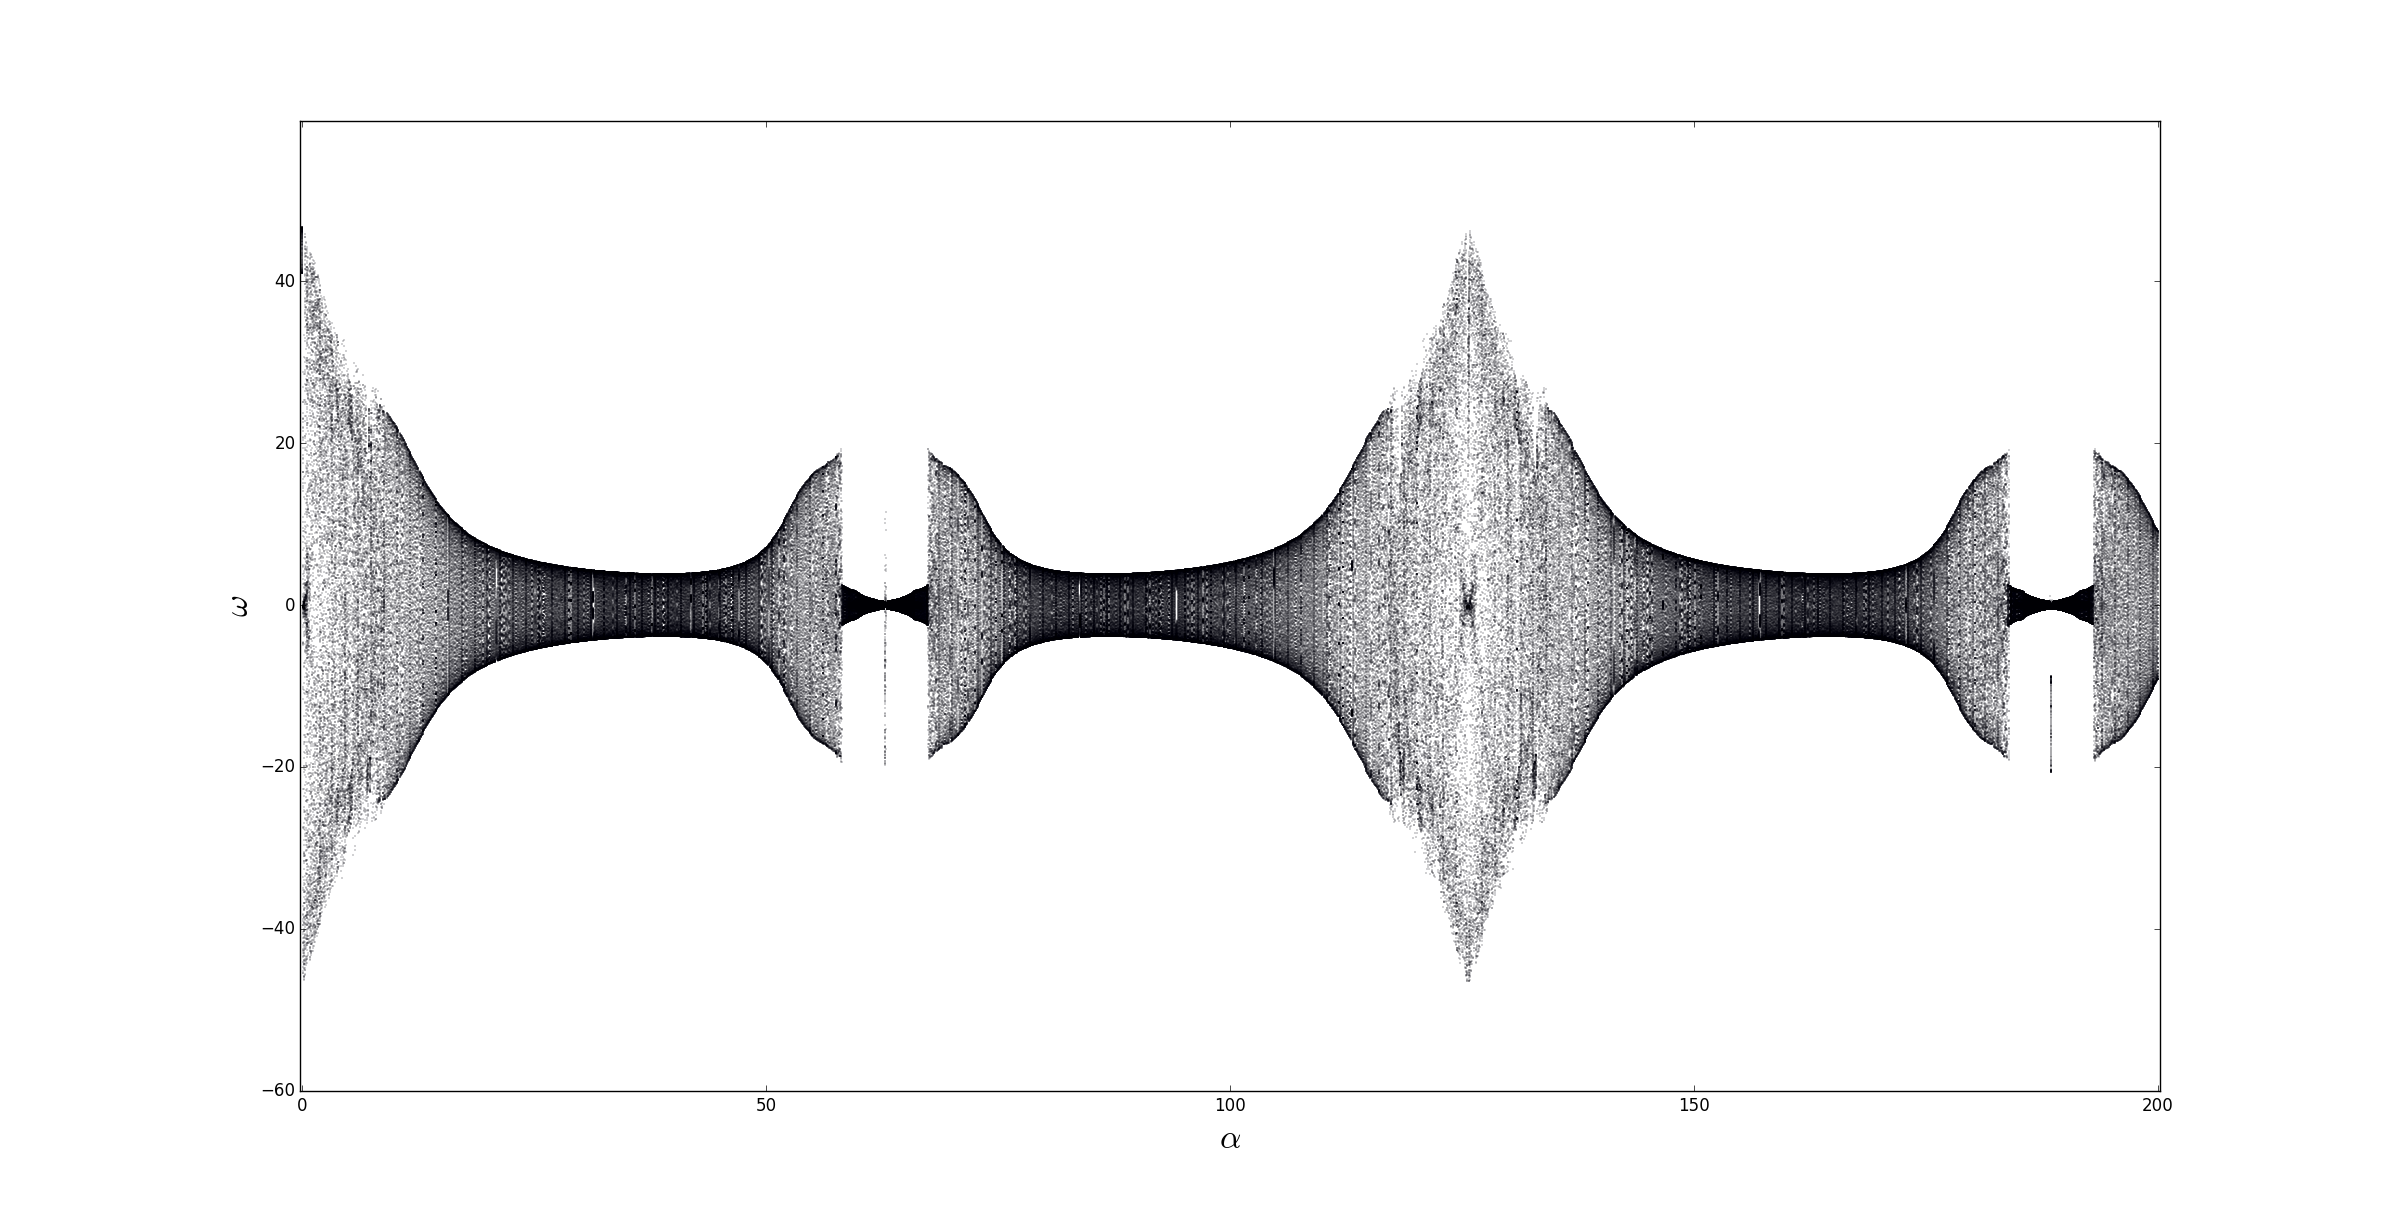
\includegraphics[scale=.25]{6_omega}
\caption{bifurcation plot of $\omega$  $g = 9.8$, $\beta = 0.0$, $m = 0.1$, $l = 0.1$,$\alpha \in [0,200]$, $A = 1.15$, step size = $0.01$}
\label{fig:my_label}
\end{figure}


If we zoom in on the beginning, we get a clear sign of bifurcations:

 \begin{figure}[H]
\centering
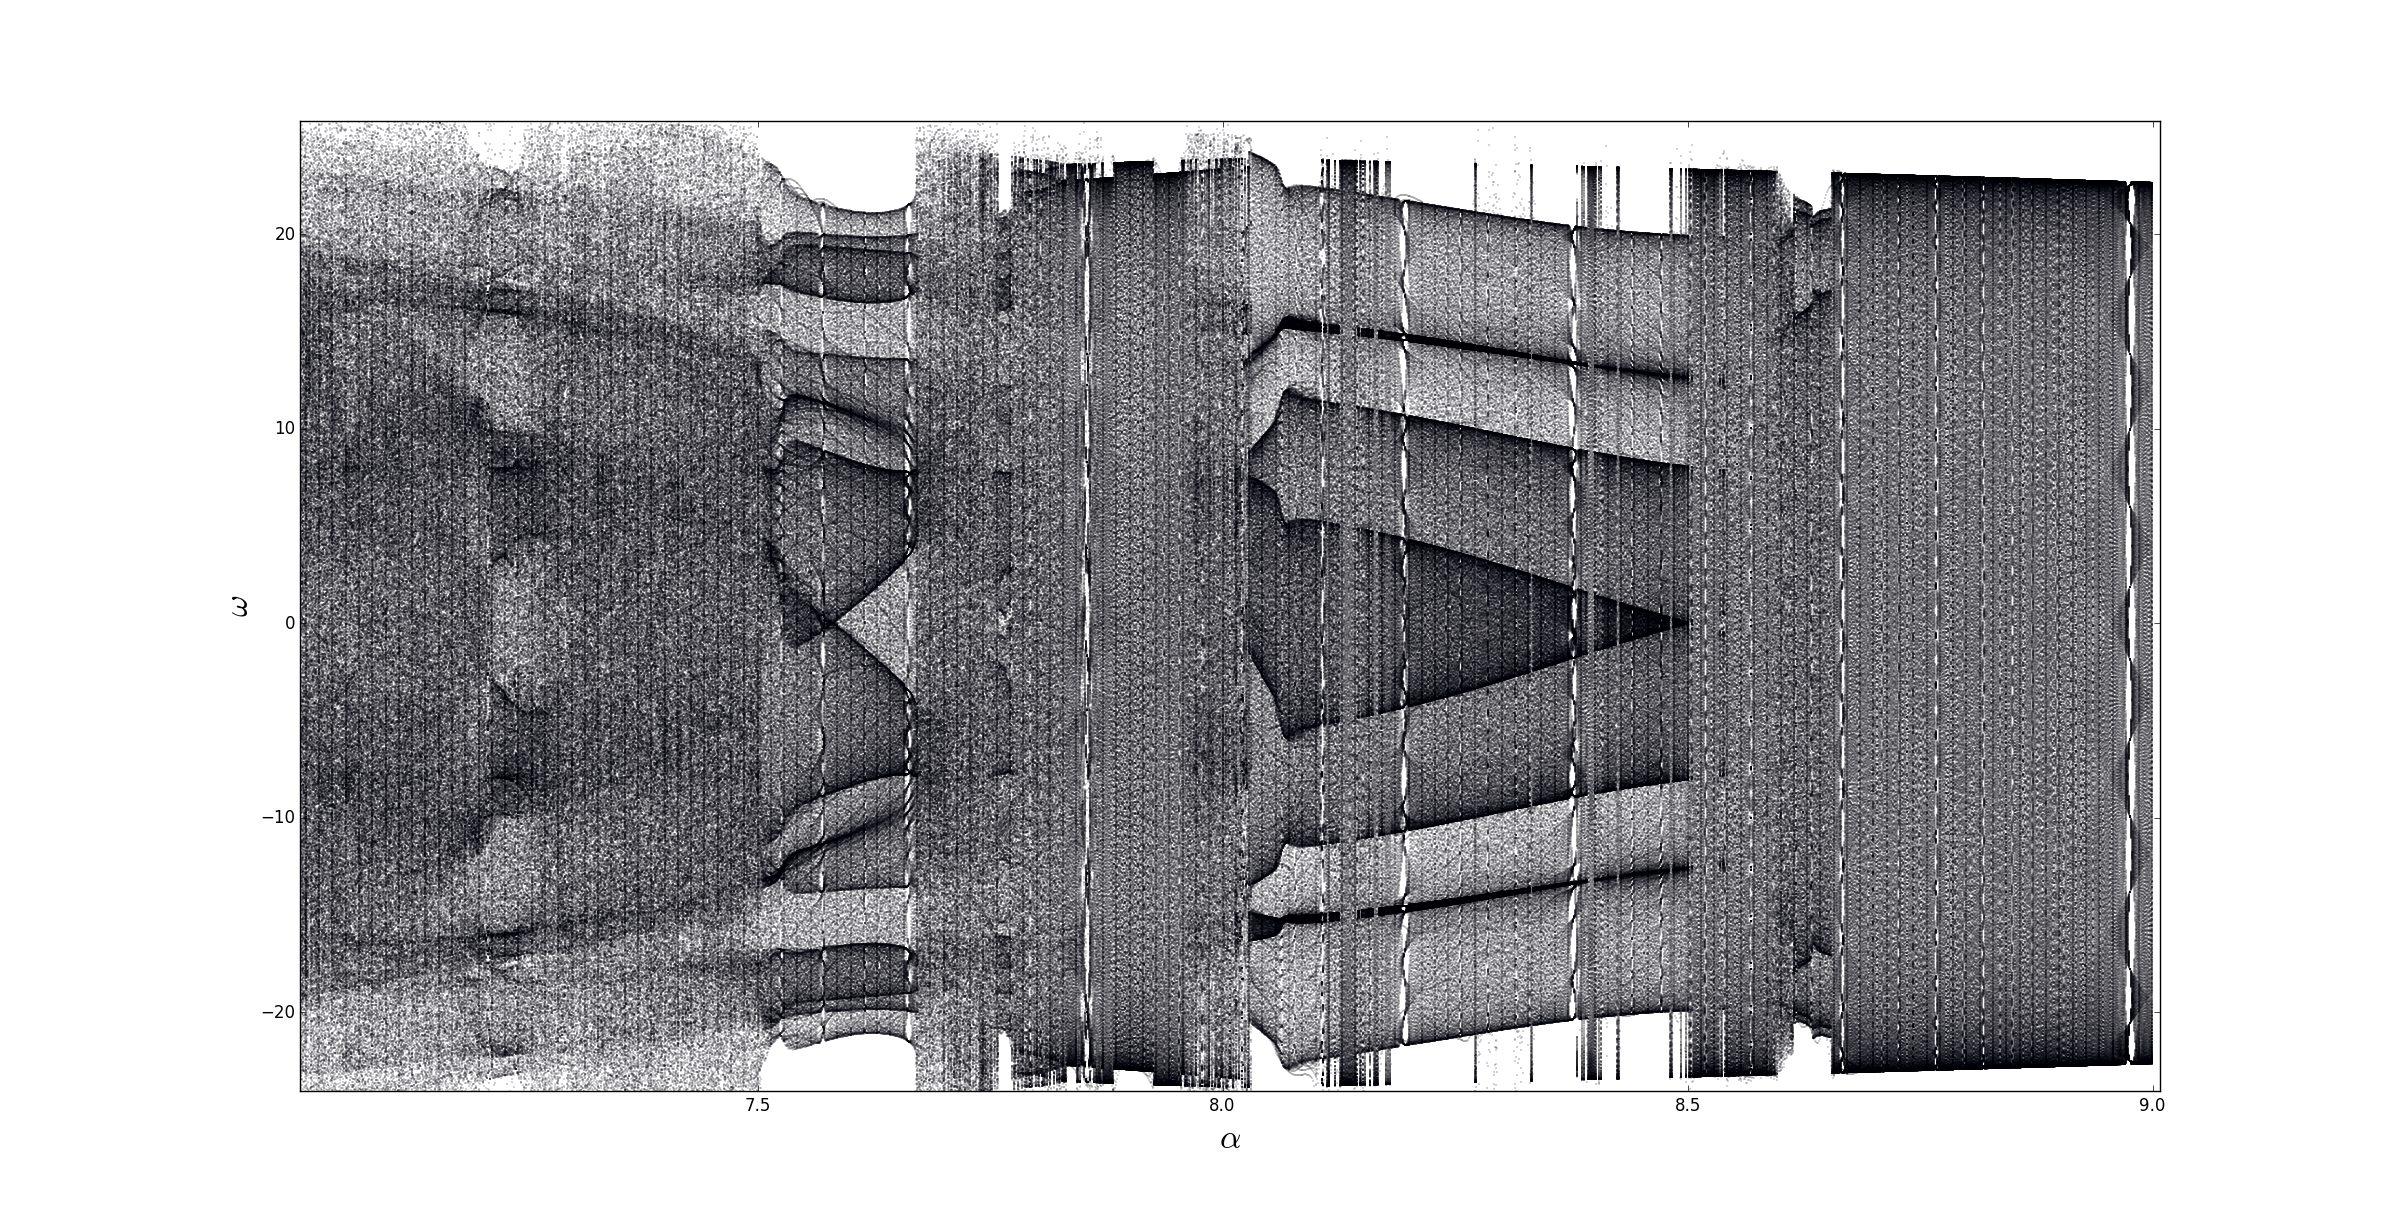
\includegraphics[scale=.20]{choosing_alpha}
\caption{bifurcation plot of $\omega$ $g = 9.8$, $\beta = 0.0$, $m = 0.1$, $l = 0.1$,$\alpha \in [0.7,0.9]$, $A = 1$, step size = $0.001$}
\label{fig:my_label}
\end{figure}

To avoid periodicity, we choose a value of $\alpha$ such that there are no clear patterns present. 

Chaos in pendulum:
7.73051559600005
 
 \begin{figure}[H]
\centering
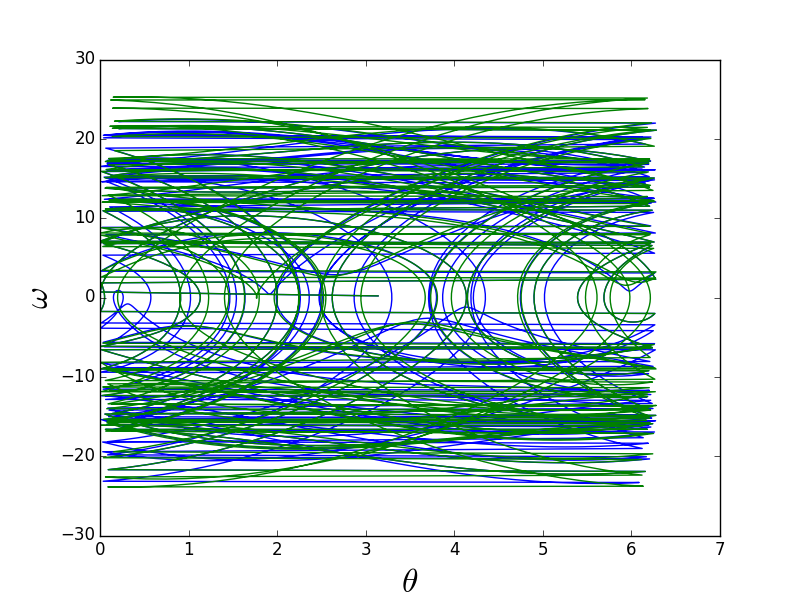
\includegraphics[scale=.5]{6_chaos_actually}
\caption{$A = 1$, $\alpha = 7.730515596$, two initial points - [3.14, 0.2], [3.14001, 0.2]}
\label{fig:my_label}
\end{figure}

Since even the slightest change in initial conditions resulted in such a drastic difference, the system is chaotic!
The result checks out with our assumption that should occur somewhere around $ 0.75 \sqrt{\dfrac{g=9.8}{l=0.1} }$.

\section{}

\begin{figure}[H]
\centering
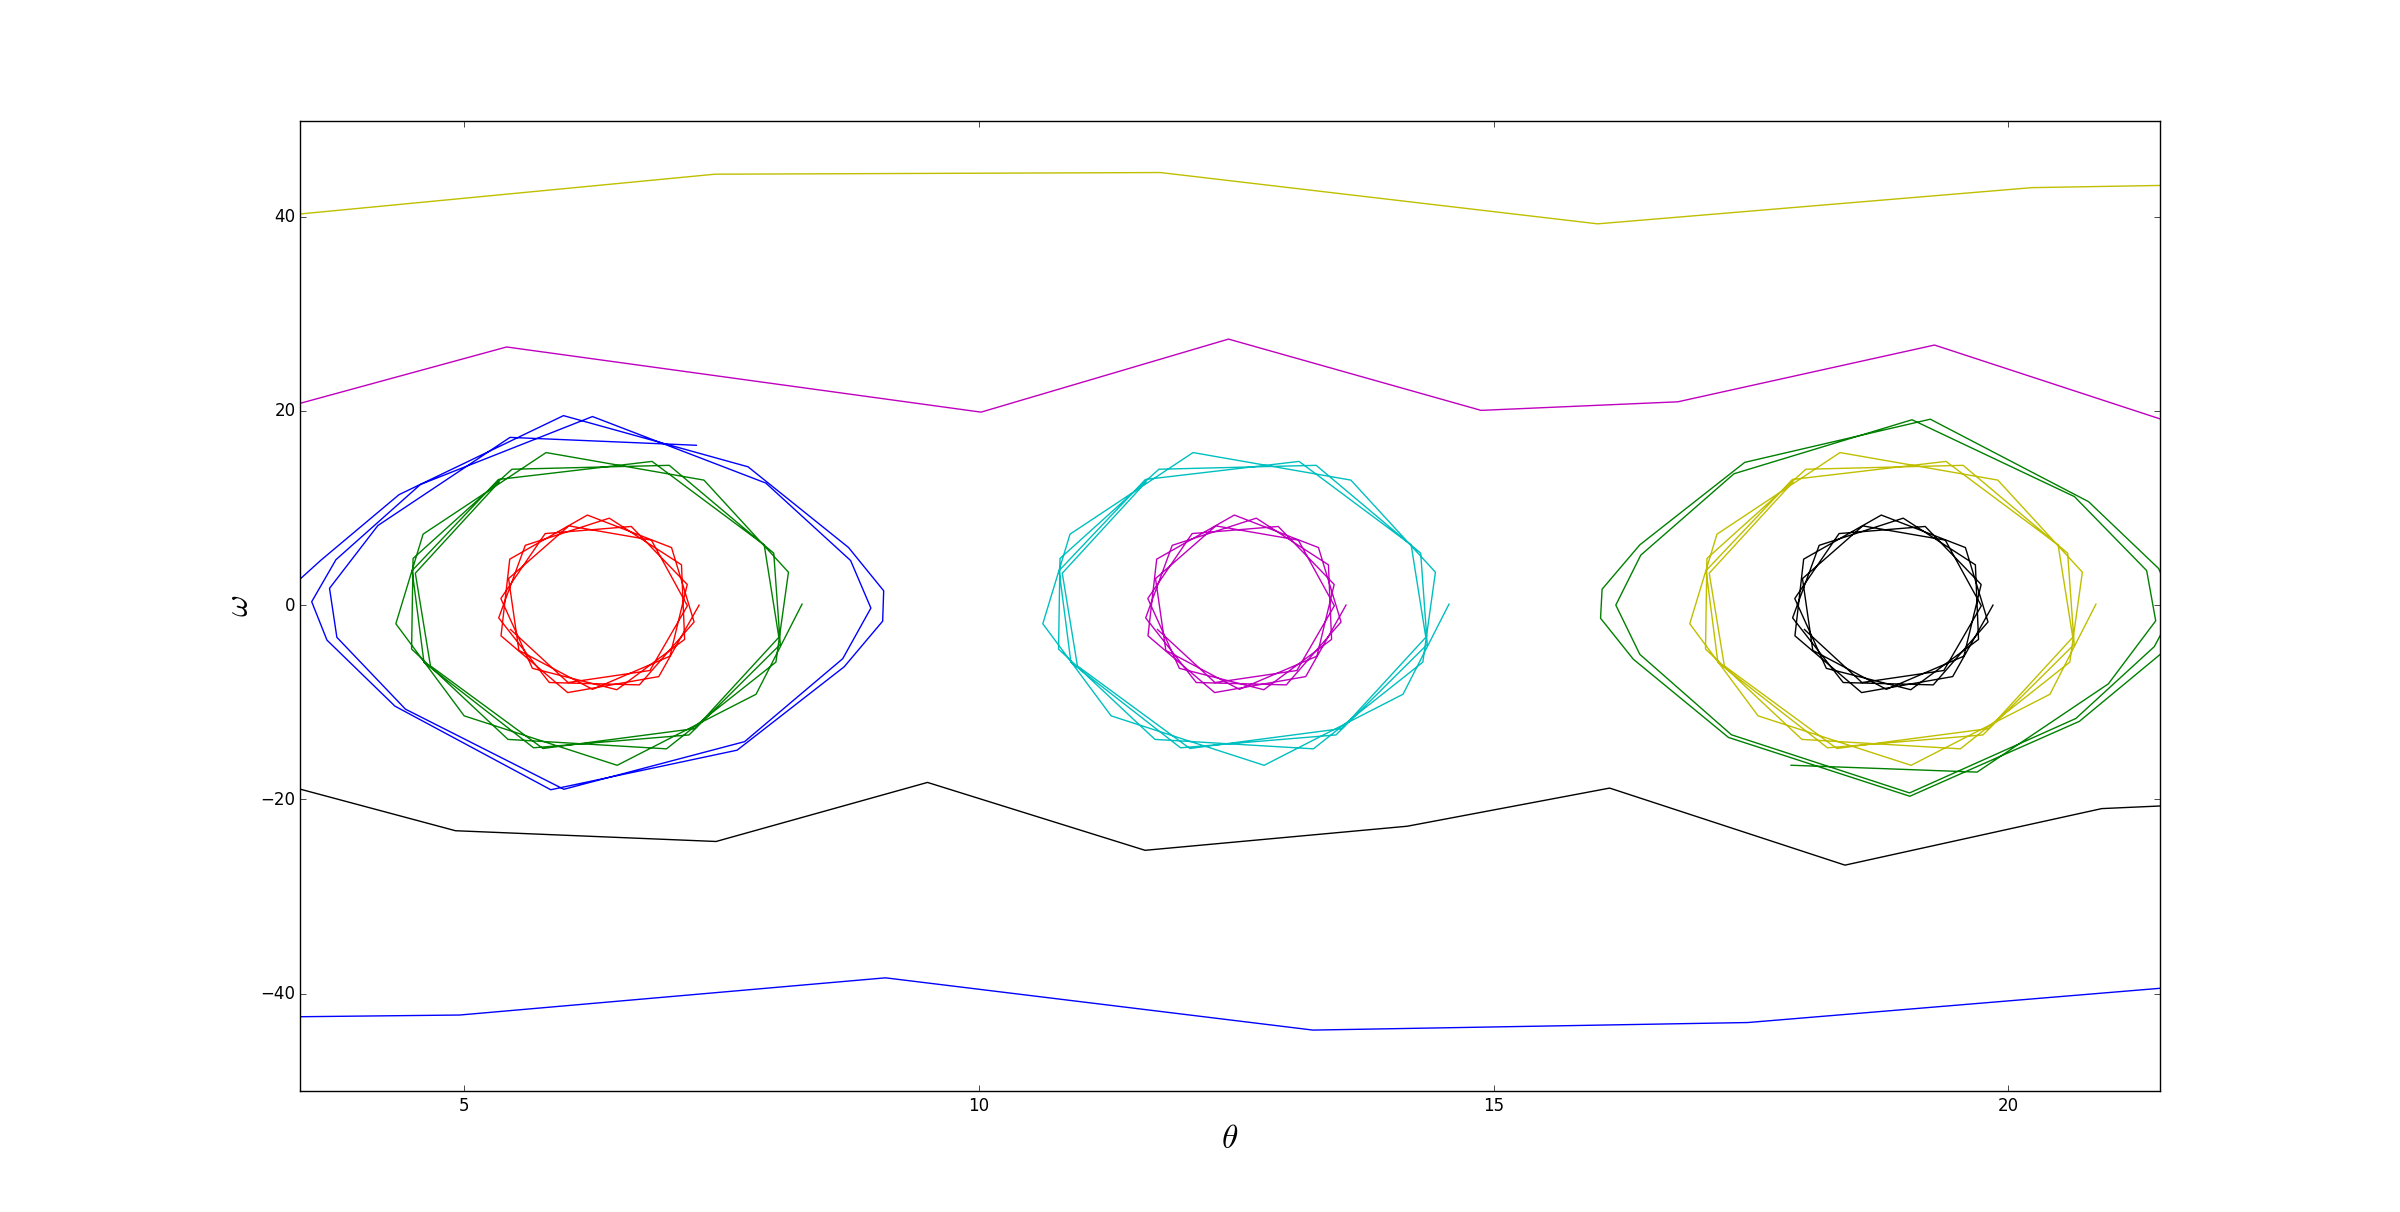
\includegraphics[scale=.15]{7}
\caption{state-space portrait using $g = 9.8$, $\beta = 0.0$, $m = 0.1$, $l = 0.1$,$\alpha = 0.0$, $A = 0.0$, step size = $0.1$}
\label{fig:my_label}
\end{figure}
We see how overall behavior of the pendulum is still preserved, but the obvious "jumps" start to get noticeable. 

\begin{figure}[H]
\centering
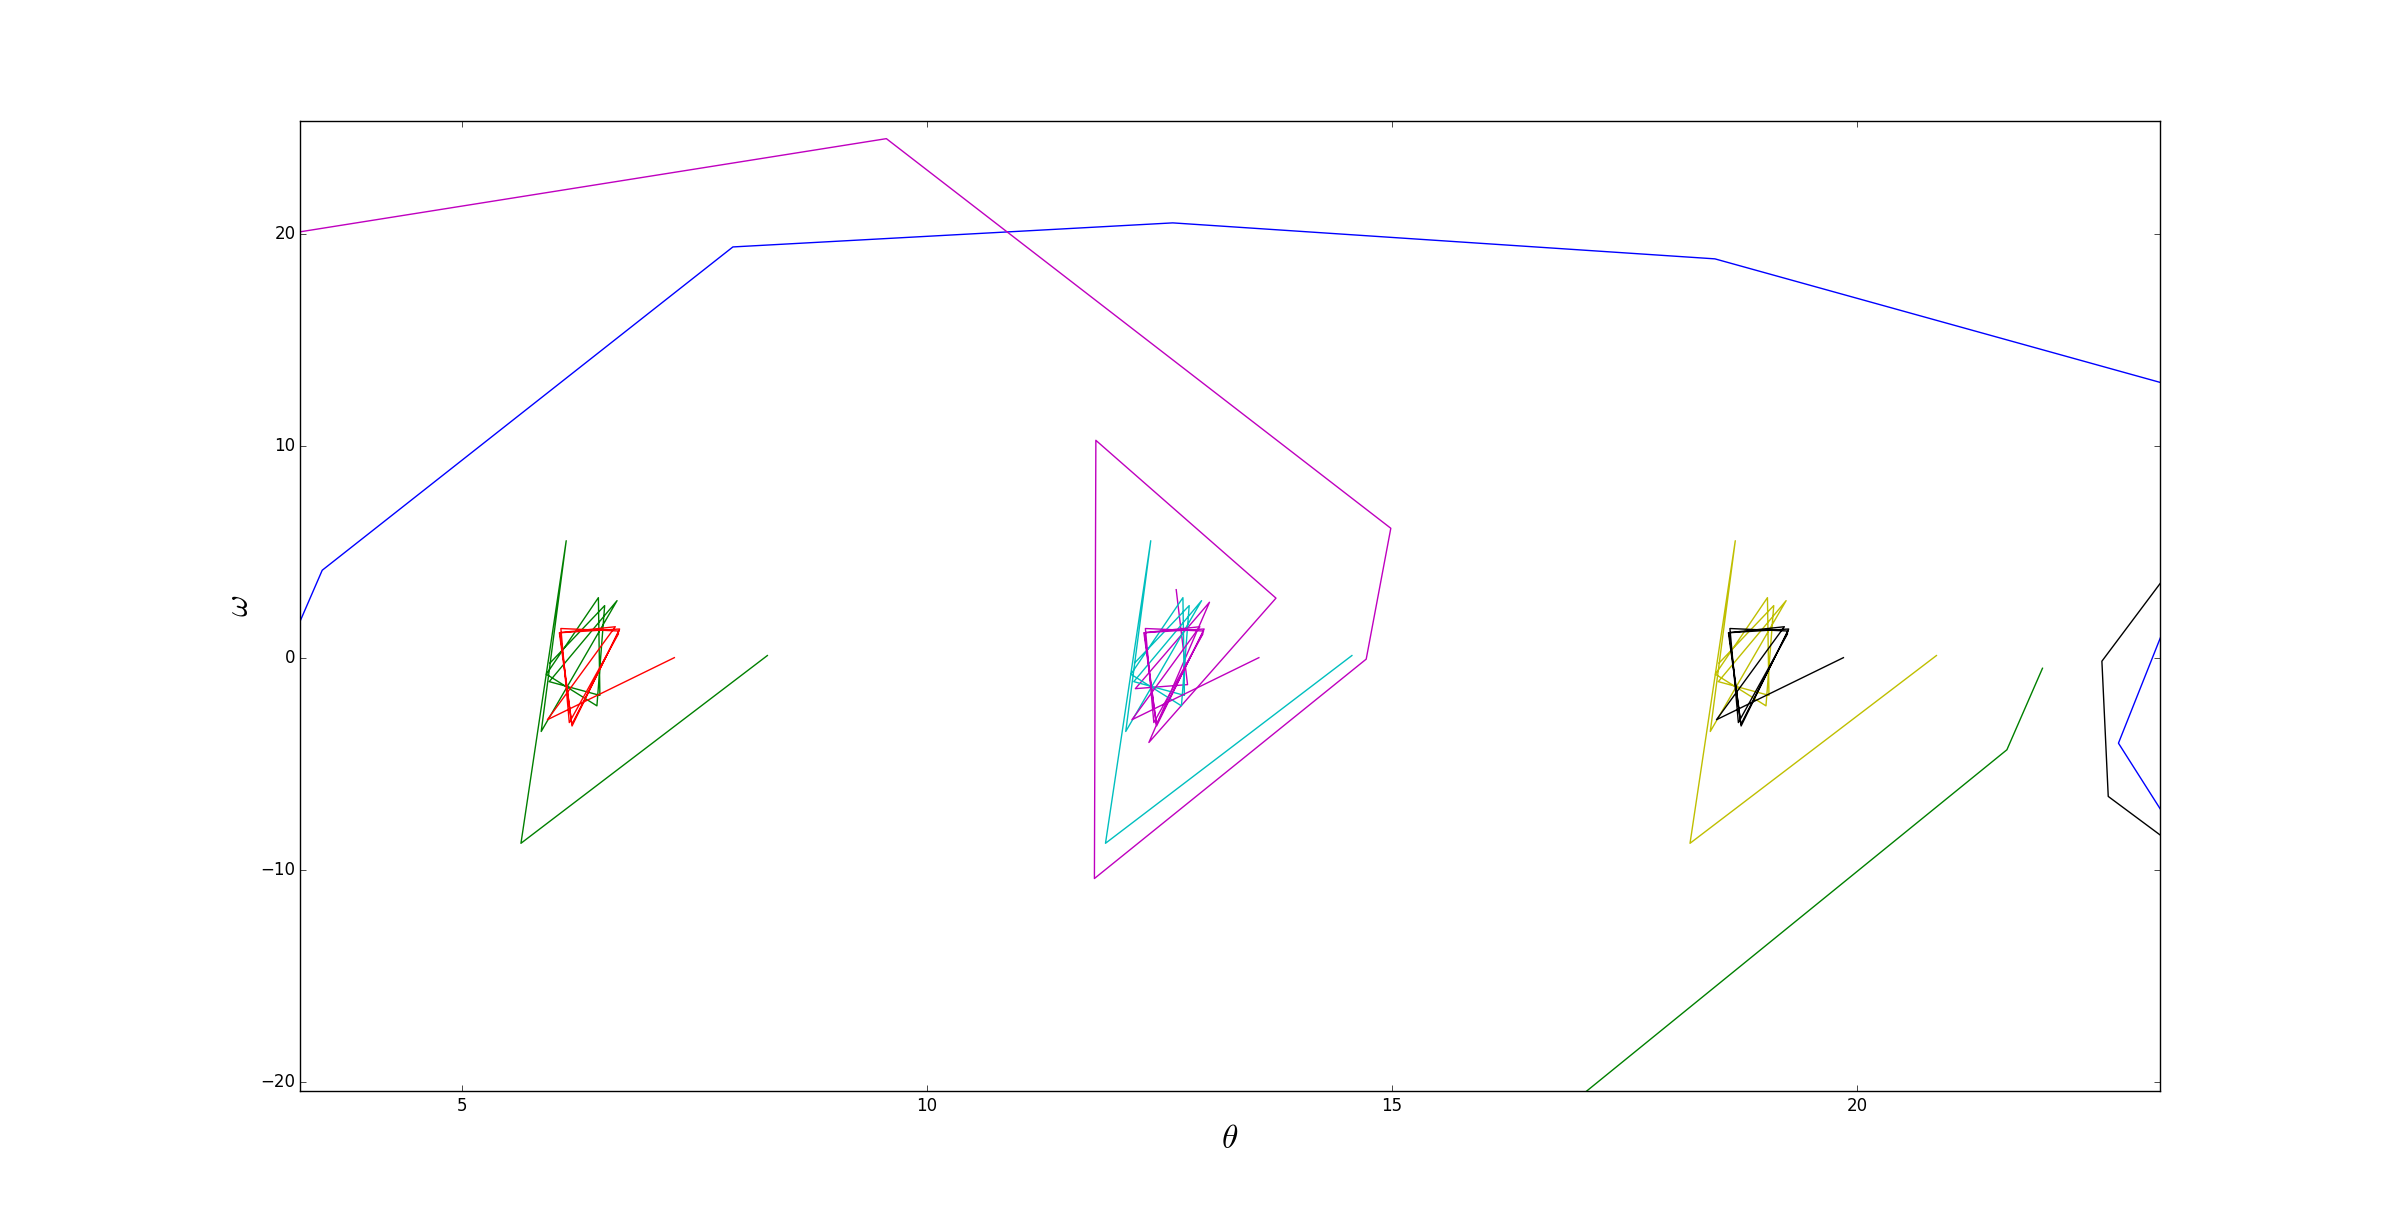
\includegraphics[scale=.15]{7_03}
\caption{state-space portrait using $g = 9.8$, $\beta = 0.0$, $m = 0.1$, $l = 0.1$,$\alpha = 0.0$, $A = 0.0$, step size = $0.3$}
\label{fig:my_label}
\end{figure}

It's easy to see how true structure becomes impossible to track as the step size gets large enough. That's because RK-4 method introduces dynamical error into its calculation, meaning that any existing error gets carried over to the next iteration and it can "snowball". In this plot it almost seems like the results "converge" to the equilibrium points, which is a dangerous deception to fall for. 

\end{document}